
%% Formato para la presentaci\'on de  proyectos de grado. 
%% Maestría en Ingeniería de Software
%% Pontificia Universidad Javeriana
%% Elaborado por Angela Villota y Luisa Rincón
%% Inspirado en Formato elaborado para carrera de Ing de Sistemas
%% V 1.0 Abril - 2022

\documentclass[12pt]{article}
\usepackage[utf8]{inputenc}
\usepackage{geometry}
\geometry{letterpaper}
\usepackage[spanish,es-tabla]{babel}
\usepackage{cite}
\usepackage{titling}
\usepackage{setspace}
\usepackage{graphicx}
\graphicspath{{img/}} %ruta de la carpeta en donde estaràn las imágenes
\usepackage{blindtext}
\usepackage{hyperref}
\usepackage{natbib} %% para citaciones
\usepackage[format=hang,font=small,labelfont=bf]{caption}

% *** ALIGNMENT PACKAGES ***
%
\usepackage{array}
\usepackage{booktabs}
\usepackage{pdflscape}
\usepackage{multirow}
\usepackage{float}
\usepackage{longtable}
\usepackage{dblfloatfix}
\usepackage{subfig}

\onehalfspacing
\setcounter{secnumdepth}{5}
\setcounter{tocdepth}{2}

\usepackage{xcolor}
\definecolor{light-gray}{gray}{0.95}
\newcommand{\code}[1]{\colorbox{light-gray}{\texttt{#1}}}

\renewcommand\maketitlehooka{\null\mbox{}\vfill}
\renewcommand\maketitlehookd{\vfill\null}


\begin{document}
%crear titulo
%\maketitle

%%%%%%%%%%%%%%%%%
% Portada del Anteproyecto
%%%%%%%%%%%%%%%%%
\begin{center}
\thispagestyle{empty}
\vspace*{0cm}
\begin{center}
    
\includegraphics[width=8cm]{pujlogo}~\\[1.75cm]
\end{center}
\textbf{\fontsize{11}{12}\selectfont
Infraestructura MLOps para despliegue o entrega continúa de un modelo de Machine Learning para el reconocimiento y control de las enfermedades Stenoma catenifer y heilipus lauri en el cultivo de aguacate Hass}\\[1.75cm]
\normalsize\textbf{Juan Felipe Rodriguez}\\[1.5cm]
\small Anteproyecto presentada(o) como requisito parcial para optar al
t\'{\i}tulo de:\\
\textbf{Magister en Ingenier\'{\i}a de Software}\\[1.5cm]
Director:\\
Ph.D. David Arango\\[1.6cm]

Pontificia Universidad Javeriana Cali\\
Facultad de Ingeniería\\
Departamento de Electrónica y Ciencias de la Computación\\
Cali, Colombia\\
\today\\
\end{center}

\newpage
%%%%%%%%%%%%%%%%%
% Ficha resumen
%%%%%%%%%%%%%%%%%
%\thispagestyle{empty}
\begin{center}
    \Large{Ficha Resumen \\ Anteproyecto de Trabajo de Grado}
\end{center}

\textbf{Posible Título:}
\begin{enumerate}
    \item Área de trabajo:
    \item Tipo de proyecto (Aplicado, Innovación, Investigación):
    \item Estudiante:
    \item Correo electrónico:
    \item Dirección y teléfono:
    \item Director:
    \item Vinculación del director:
    \item Correo electrónico del director:
    \item Co-Director (Si aplica):
    \item Grupo o empresa que lo avala (Si aplica):
    \item Otros grupos o empresas:
    \item Palabras clave(al menos 5):
    \item Fecha de inicio:
    \item Duración estimada (en meses):
    \item Resumen:  Debe contener el tema a trabajar en el proyecto de grado, su importancia, la problemática que aborda, los objetivos propuestos, resultados esperado y posibles aplicaciones.  Debe ser redactado en un solo párrafo y no contener espacios entre líneas ni sangría.  Debe ser escrito con máximo 400 palabras 
\end{enumerate}

%\newpage

%%%%%%%%%%%%%%%%%
% Indices y tablas
%%%%%%%%%%%%%%%%%

\tableofcontents
%\listoffigures
%\listoftables
\newpage

%%%%%%%%%%%%%%%%%
% Resumen / abstract
%%%%%%%%%%%%%%%%%
%%%%%%%%%%%%%%%%%
% ABSTRACT
%%%%%%%%%%%%%%%%

\section*{Resumen}
Resumen en Inglés
150 palabras aprox

Esimula la capaidad de síntesis del autor. Puede ser más fácil de escribir al finalizar el anteproyecto pues en este punto el autor tiene mejor comprensión de su propuesta y del alcance que está tiene. 

No incluye citas o referencias bibliográficas.


\paragraph*{}{\textbf{Palabras Clave}}
entre tres y cinco palabras que diferencien su trabajo. Son las palabras que van a facilitar que tu documento sea visible en cualquier motor de búsqueda. Piense en palabras que describan las ideas principales del proyecto. Un conjunto de palabras clave asociadas a Ciencias de la computación se puede encontrar en \url{https://dl.acm.org/ccs}
\section*{Abstract}
Summary 
Around 150 words. 
\paragraph*{}{\textbf{Keywords}}
 
%\newpage

%%%%%%%%%%%%%%%%%
% Introduccion
%%%%%%%%%%%%%%%%%
%\section{Introducción}

Aquí algunos ejemplos de como se usan las imágenes, las tablas las listas

\textbf{ text in bold}
\textit{text in italics}
\underline{underlined text}
\texttt{text in consola-like font}

\subsection{Ejemplos de listas}
itemize, enumerate, description

\subsubsection{Viñetas}
\begin{itemize}
    \item cada item es una viñeta
    \item Otra viñeta
\end{itemize}

\subsubsection{Números}
\begin{enumerate}
    \item enumeración
    \begin{enumerate}
        \item anidado
    \end{enumerate}
\end{enumerate}

\subsubsection{Etiquetas}
\begin{description}
    \item[etiqueta1] texto asociado a la etiqueta
    \item[etiqueta2] otro texto
\end{description}



\subsection*{Uso de figuras ambiente figure}
La Figura \ref{fig:figure1} muestra un gráfico de ejemplo. Las tablas y figuras que aparecen en el documento deben ser previamente introducidas y explicadas


\begin{figure}
\centering
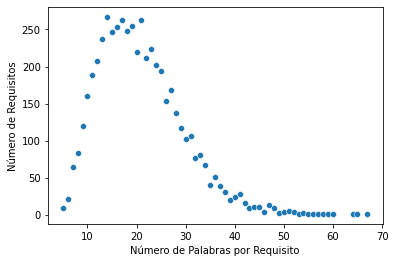
\includegraphics[width=0.5\textwidth]{freq_req.png}
\caption{Grafico tridimensional. Elaboración propia}
\label{fig:figure1}
\end{figure}

\begin{figure*}[htb]
\centering
\subfloat[] {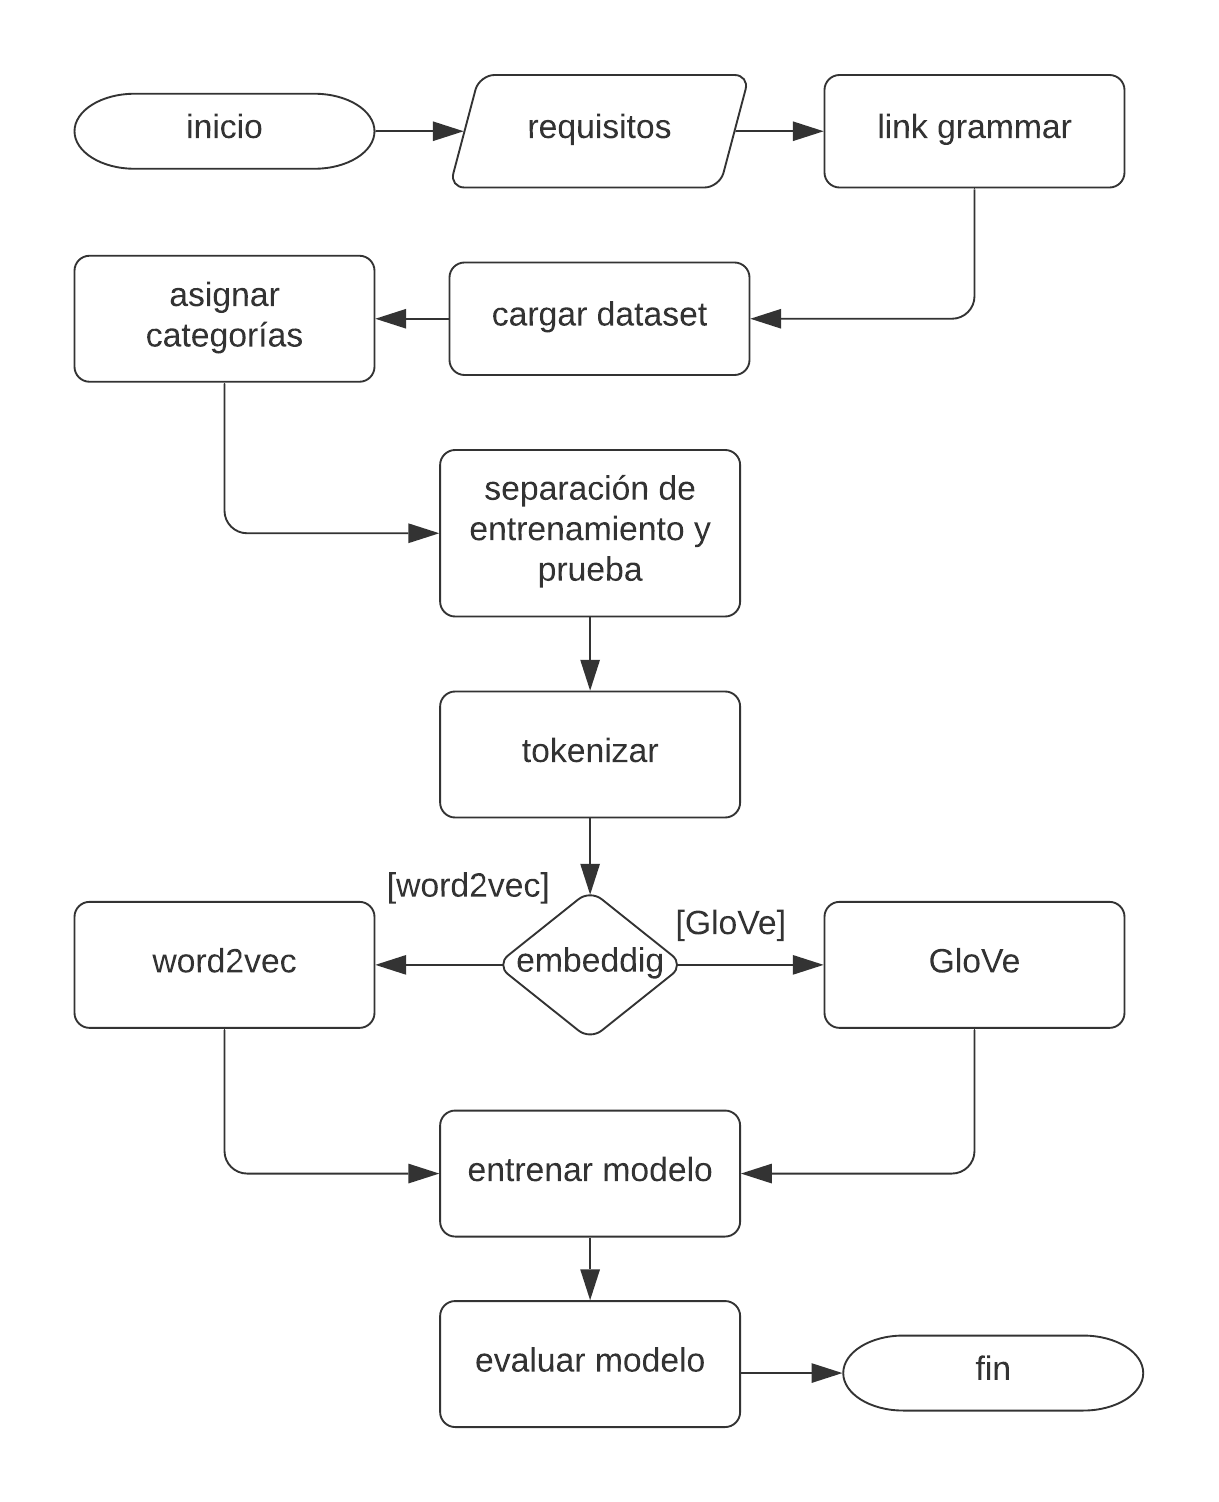
\includegraphics[width=0.5\textwidth]{Deep.png}

\label{fig:PAS_FM}}
\subfloat []{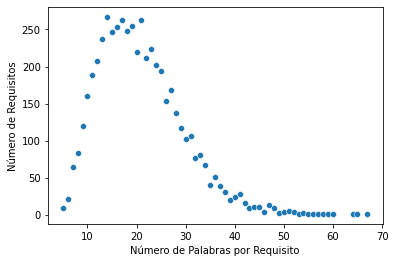
\includegraphics[width=0.38\textwidth]{freq_req.png}

\label{fig:PAS_FM2}}

\label{fig:examples}
\end{figure*}

 \subsection*{Uso de tablas, ambiente table y tabular}
 \begin{table}[htb]
     \centering
     \begin{tabular}{rc} 
	\toprule
    	Item1 & Item2  \\ % --> salto de línea 
	\midrule
	celda 1 & celda 2\\
	\bottomrule

\end{tabular}
     \caption{Propuesta de elementos identificados en el desarrollo del proyecto. Fuente \citep{Hinton2012}}
     \label{tab:my_label}
 \end{table}

 
%\newpage

%% Problema
\section{Definición del problema}
% Un problema es todo aquello cuya solución se desconoce; ese desconocimiento puede ser para un grupo de personas o para la humanidad. Para la formulación correcta de un problema se debe tener en cuenta los siguientes aspectos:
 
% \textcolor{red}{Como decía \citet{Glorot2011} el trabajo deberia hacerse de la siguiente manera:} 

\subsection{Planteamiento del problema}
Los aportes económicos, laborales, alimenticios y sociales de los procesos agrícolas son fundamentales para el desarrollo de un país, situación que pone de manifiesto la mirada de los entes gubernamentales y no gubernamentales internacionales y nacionales en el renglón de la economía agrícola y de la comunidad que se encuentra articulada en este ámbito económico.\\ 

La producción agrícola del aguacate Hass para el caso de México en el año 2019 correspondió a un 2.4 millones de toneladas, aportando el 45\% en las exportaciones de este país y aumentando la cantidad de exportaciones en un 22\% en el año 2020 \citet{cruz2022competitividad}. Estos aportes a nivel nacional se reflejan en PIB, contribuyendo al avance socioeconómico de las regiones agrícolas.\\

El aguacate Hass corresponde cerca del 82\% de todos los aguacates el más consumido a nivel mundial. De acuerdo con los datos de la Organización de las Naciones Unidas para la Alimentación y la Agricultura \citet{faostat2021hacia} el primer país productor de aguacate Hass es México con unas 2.393.849 toneladas al año, seguido de Colombia con unas 876.754 toneladas al año y de República Dominicana con 676.373 toneladas al año.\\

Los avances en la agroindustria en Colombia contribuyen al ámbito económico y laboral, siendo en la actualidad la producción agrícola del cultivo de aguacate hass un producto de alta demanda a nivel nacional e internacional. Para el Departamento Administrativo Nacional de Estadística \citet{dane2016cultivo}, Las problemáticas a tener en cuenta en el cultivo del aguacate Hass corresponden a: factores atmosféricos relacionados con la temperatura, las precipitaciones, el viento, la altitud, los factores de las condiciones del terreno y los factores relacionados con la siembra donde se encuentra la fertilización, los abonos y el tratamiento de las plagas y enfermedades.\\

Dentro de las enfermedades más importantes en el cultivo del aguacate Hass se encuentran 
la Stenoma catenifer y el heilipus lauri, insectos y larvas que introducen sus huevos provocando el daño en las semillas de los frutos en crecimiento. Además, el Stenoma catenifer impacta en el fruto al perforar el brote terminal y los laterales del aguacate, formando túneles de hasta 25cm, corta los pedúnculos y la base de los frutos pequeños, como resultado los frutos verdes y pequeños caen.\\

Para prevenir y controlar estas enfermedades, se recomienda implementar prácticas agrícolas adecuadas, como el manejo integrado de plagas, la selección de variedades resistentes y el control de la humedad en el suelo. Además, se deben realizar monitoreos constantes para detectar y tratar a tiempo cualquier enfermedad que pueda aparecer en el cultivo del aguacate Hass.\\

Para la detección de este tipo de plaga en la producción agrícola del cultivo del Hass existe el método Manejo Integrado de Plagas (MIP) en el cual se señala el monitoreo de manera manual y de observación constante partiendo de tres elementos, el primero corresponde a la prevención como cuidados, restricciones y limpieza del personal y sus utensilios de trabajo, el segundo al control donde se utiliza evaluaciones y registros manuales, instalación de trampas y el tercero es el manejo de la enfermedad en el cual se genera una protección y cuidado de las plantas dependiendo de los patógenos dañinos \citet{ica2012manejo}.\\

En este sentido el Machine Learning permite a través de imágenes el reconocimiento de patrones de concentración y expansión de las plagas de manera óptima en todo el cultivo generando una reducción económica y mejorando la calidad del producto agrícola.\\\\

El cultivo del aguacate Hass en Colombia ha tenido una gran demanda a nivel nacional e internacional, generando un crecimiento del 34\% del total de área sembrada de aguacate, además al ser un producto que presenta una cosecha constante por las condiciones del relieve y climáticas del país viene en un crecimiento de área sembrada de un 65\% (Ministerio de Agricultura y Desarrollo Rural, 2021). Por esta razón, la metodología MLOps puede mejorar la calidad, la confiabilidad y la eficiencia de los modelos de machine learning a encontrar el tipo de plaga, la cantidad de daño, identificando procesos de deformación y tipos de coloraciones especificas del área afectada, debido a que los modelos están sujetos a rigurosos procesos de control de calidad y proporciona trazabilidad y transparencia en todo el ciclo de vida del modelo.\\

La utilización de MLOps se ha convertido en una práctica cada vez más extendida en el campo de la ciencia de datos, y se ha demostrado que mejora significativamente la eficiencia y efectividad en la implementación de modelos de Machine Learning \citet{geron2019hands}. Su aplicación en el contexto de la agricultura y la predicción de enfermedades puede ser un paso importante para mejorar la productividad y sostenibilidad del cultivo de aguacate Hass y otros cultivos.\\

Es importante destacar la relevancia de utilizar prácticas de MLOps para garantizar el correcto desarrollo, implementación y mantenimiento continuo de un modelo de control y cuidado de plagas permitiendo mejorar los procesos productivos agrícolas en Colombia. El modelo de Machine Learning al ser un programa de automatización y actualización constante de sus tareas avanza en el mejoramiento y la eficiencia de su procesamiento de información de manera continua a través de la metodología MLOps.
\\\\



% \textbf{TIP:} Contexto + antecendents  + situación problema
% \textit{qué} o \textit{cómo}

\subsection{Formulación del problema}
En este contexto la investigación busca desarrollar una herramienta digital que ayude a pronosticar y prevenir la posible la presencia o no de las enfermedades como el Stenoma catenifer y el heilipus lauri en el cultivo de aguacate Hass, entendiendo que es crítico la detección temprana y continua del brote en un cultivo y por lo tanto la solución debería estar disponible en un software para los científicos de datos, de allí que se planteó la siguiente pregunta de investigación ¿Cómo el uso de MLOps para desarrollar un modelo de Machine Learning permite la integración, la actualización y el despliegue continuo del reconocimiento de las enfermedades Stenoma catenifer y heilipus lauri en el cultivo de aguacate Hass, contribuyendo a mejorar los modelos agrícolas de forma automática y brindando beneficios económicos y sociales a la comunidad de científicos de datos? asimismo ¿Cómo mantener el programa de Machine Learning de manera automatizada y de supervisión continua de manera que no pierda rendimiento?

\newpage

%% Objetivos
\section{Objetivos del proyecto}
% Los objetivos deben formularse de manera que logren transmitir lo que intenta realizar el investigador y lo que espera obtener como resultado. 

% Los objetivos deben iniciar con un verbo en infinitivo (construir, diseñar, seleccionar, analizar, modelar simular, etcétera.) 

% En resumen el objetivo general responde \textbf{¿qué se espera lograr con el proyecto de grado?}


\subsection{Objetivo General}
Diseñar e implementar una infraestructura MLOps para el despliegue o entrega continua de un modelo de Machine Learning para el reconocimiento y control de las enfermedades Stenoma catenifer y heilipus lauri en el cultivo de aguacate Hass.




\subsection{Objetivos específicos}
\begin{itemize}
  \item Desarrollar una infraestructura MLOps que permita la integración, automatización y monitorización del modelo de machine learning para el reconocimiento y control de las enfermedades Stenoma catenifer y heilipus lauri en el cultivo de aguacate Hass.
  \item Validar el uso de MLOps mediante despliegue en un ambiente controlado, con la capacidad de monitorear y mejorar continuamente el rendimiento del modelo.
  \item Desarrollar y entrenar un modelo de Machine Learning utilizando técnicas apropiadas de preprocesamiento y selección de características, así como algoritmos de aprendizaje supervisado o no supervisado, para lograr una detección de las enfermedades Stenoma catenifer y heilipus lauri en el cultivo de aguacate Hass.
  \item Implementar técnicas de procesamiento de imágenes para extraer características relevantes y mejorar la capacidad del modelo de Machine Learning en el reconocimiento y detección de las enfermedades Stenoma catenifer y heilipus lauri en el cultivo de aguacate Hass a partir de imágenes capturadas en campo.
\end{itemize}



%\subsection{Resultados esperados}
%Los resultados esperados se redactan teniendo en cuenta los objetivos de investigación, el problema que se quiere investigar, y las posibilidades reales de producir los mismos reconociendo las condiciones en que puede operarse o ejecutarse el proyecto de investigación.
\newpage

%% Alcance
%\section{Alcance}
Se analiza cada objetivo específico, buscando delimitar con mayor precisión qué se va a hacer y qué no.
Deja claras limitaciones ya identificadas en la solución que se va a construir.
Identifica algunos obstáculos que eventualmente pudieran presentarse durante el desarrollo de la investigación.
Define hasta dónde llegará el trabajo.

%\newpage

%% Justificacion
%\section{Justificación del trabajo de grado}
Este texto explica porque la solución contribuye a mejorar las condiciones adversas de los afectados en forma negativa por el problema. Explica ¿qué pasaría si SI se resuelve el problema de investigación?

Se suele redactar en términos de impactos, contribuciones positivas para generar nuevo conocimiento o experiencias. 

Explica qué beneficios genera la solución del problema, por ejemplo en lo económico, social, ambiental, etc a los afectados negativamente por el problema.

¿Qué impactos y beneficios genera la solución del problema, en lo económico, social, ambiental, etc.? 

\textbf{Nota:} Respalde las afiramaciones con evidencias y hechos verificables que hayan sido documentados a través de publicaciones científicas y/o ingeniería. 

%\newpage

%% Marco conceptual
%\section{Marco teórico de referencia y antecedentes}
Es una recopilación de información de todo aquello que se haya hecho alrededor del tema propuesto. Sirve como una orientación acerca del enfoque que debe darse al proyecto, porque al acudir a los antecedentes, el proponente puede darse cuenta de cómo ha sido tratado el problema: qué tipos de estudio se han efectuado sobre él, qué modelos y diseños se han utilizado, dónde y cómo se han recolectado los datos, etc. 

\textbf{La construcción del estado del arte sirve como punto de partida para la realización del proyecto.}

Para el anteproyecto se recomienda una extensión de máximo 10 páginas para esta sección.

\subsection{Bases Teóricas}
En esta sección se describen los fundamentos teóricos que sustentan el trabajo de investigación o proyecto de grado, con sus respectivas citas bibliográficas (Es muy importante el manejo riguroso de las citas). 

Tenga encuenta la siguiente lista de chequeo:
\begin{itemize}
    \item Los temas tratados en el marco teórico deben ser relevantes al problema que se está abordando. Estas descripciones no deben ser demasiado extensas ni repetir la teoría que está en los libros, debe presentar los conceptos fundamentales y hacer referencias a libros o artículos donde esos temas se tratan con mayor detalle. 
    \item Los temas aquí abordados deben ser relevantes con el fin de hacer el documento autocontenido.
    \item NO asuma que el lector es un experto 
    \item NO se trata de una enumeración de
fuentes y conceptos aislados, sino de que presenta de manera artículada los conceptos relevantes para entender la investigación. 
\item Use las definiciones de los autores "seminals" o los autores referentes del área. 
\end{itemize}

Tips de lo que no va:
\begin{itemize}
\item  NO incluir material que el lector no necesita para entender lo que sigue
\item  No incluya material que no se conecta con alguna sección de la tesis
\item NO incluya temas que rompan el flujo del argumento. Algunas cosas pueden parecer importantes pero podrían ser Anexos. 
\end{itemize}

\subsection{Estado del Arte}
Esta sección da cuenta del estado en el que se encuentra la investigación sobre el tema que se está explorando con el proyecto de grado. Tiene como objetivo revisar y analizar el conocimiento acumulado alrededor del problema, y evidenciar cuál es el estado actual de la solución a un problema respecto al problema que se desea abordar. 

Esta sección presenta trabajos previos (estudios o implementaciones) que abordan el problema de forma similar, da confianza sobre el conocimiento del autor de referentes anteriores así como permite que no se repitan estudios sobre asuntos explorados previamente.

\textbf{Nota:} \textit{En el anteproyecto este análisis puede ser más superficial pero a medida que lo haga mejor podrá reutilizar más para su documento final.}

\subsubsection*{¿Qué incluir?}
Piense en los siguientes temas:
\begin{itemize}
    \item ¿Cómo se ha resuelto el problema?
    \item ¿Quienes han resuelto el problema?
    \item ¿Qué aspectos técnicos económicos, culturales normativas estándares se han tenido en cuenta?
    \item ¿El problema ha sido resuelto en otro contexto?
\end{itemize}

\subsubsection*{¿Qué NO debe incluir?}
\begin{itemize}
    \item NO incluya ideas propias o reflexiones respecto a cómo solucionar el problema. Facts only. 
    \item NO describa información de otros trabajos o problemáticas que usted NO va a abordar 
\end{itemize}

\subsubsection*{¿Cómo organizarlo?}
\begin{itemize}
    \item Definición de un conjunto de criterios que van a usarse para comparar los trabajos de otros
    \item Una descripción corta de cada propuesta - previas de solución del problema. Resalte en cada una ventajas y desventajas. 
    \item  Indique de forma clara: ¿Por qué las propuestas y soluciones revisadas no sirven en el contexto del estudio y porque no resuelven la pregunta planteada en su proyecto de investigación?
    \item \textbf{DESEABLE}: haga tablas o gráficas que presenten cuál es el vacío que tiene la situación actual. 
\end{itemize}



%\newpage

%% Metodología
%\section{Metodología de la investigación}
La metodología debe reflejar la estructura lógica del proceso de investigación. Esta sección define y explica la selección de la estrategia adoptada para responder al problema planteado y además explica el cómo va a realizar la investiga. 

La metodología indica cómo será el proceso desde la recolección de los datos, la organización, sistematización, y análisis de la información, hasta la forma como se van a interpretar y presentar los resultados.   Si bien esto puede cambiar en la realización del proyecto una metodología concreta permite tener una guía para la elaboración del proyecto. 

La metodología definida debe reflejar la articulación entre los objetivos, el proyecto y los procedimientos para cumplir dichos objetivos. 


%\newpage

%% Recursos
%\section{Recursos a emplear}
Esta sección resume los recursos que van a emplearse en el desarrollo del proyecto de grado. Los recursos que deben considerarse incluyen a las personas que estarán involucradas en el proyecto y a los materiales como licencias, libros, etc.  A continuación se listan los posibles recursos que se requieren en un proyecto de grado.
\begin{enumerate}
    \item Recursos Humanos
    \begin{enumerate}
        \item Director
        \item Co-Director (si existe)
        \item Asesor (si existe)
        \item Grupo de Investigación de la Facultad que lo avala
        \item Otros grupos
    \end{enumerate}
    \item Económicos
    Presupuesto General de recursos requeridos (materiales, insumos, equipos, software y material bibliográfico)
\end{enumerate}
%\newpage

%% Cronograma
%\section{Cronograma de actividades}
%\newpage

\section{Referencias Bibliográficas}
%Se deben presentar de forma rigurosa y completa las referencias bibliográficas utilizadas en el documento (No incluir bibliografía no referenciada en el documento). Se debe seguir una sola norma de referenciación en todo el documento, ej. IEEE, Harvard o APA.

%Utilizar en lo posible bibliografía reciente de fuentes confiables y en inglés(libros, artículos científicos, etc.). Evitar utilizar fuentes no confiables como blogs, Wikipedia, o documentos sin autor.
%\bibliographystyle{IEEEtran}
\bibliographystyle{apalike}
\bibliography{bibfile}
\newpage

%\section{Glosario de Términos}
%Esta sección presenta un conjunto de definiciones cortas de términos que se usan en el documento del proyecto.  A continuación se presenta un extracto de un glosario de términos tomado de la tesis de ...

% \begin{description}
% \item[Accuracy] Métrica del porcentaje de clasificaciones correctas de un modelo de
% aprendizaje supervisado.
% \item[Bootstrap] En el contexto del aprendizaje de conjuntos de hipótesis,
% es el uso de un subconjunto aleatorio de atributos y datos de entrenamiento obtenido
% a partir de los datos originales, con esto se espera reducir la posibilidad de
% \emph{overfitting}.
% \item[Corpus] Un corpus lingüistico es un conjunto amplio de ejemplos reales del uso de un
% lenguaje.

% \end{description}





\end{document}
